% \VignetteIndexEntry{basic examples of mixed stock analysis}
\documentclass[11pt]{article}
\usepackage{palatino}
\usepackage[american]{babel}
\newcommand{\R}{{\sf R}}
\newcommand{\Splus}{{\sf S-PLUS}}
%\newcommand{\fixme}[1]{\textbf{FIXME: #1}}
\newcommand{\fixme}[1]{}
\usepackage{url}
\usepackage{alltt}
\bibliographystyle{plain}

\newcommand{\Rver}{2.4.1}
\title{Mixed stock analysis in R: getting started with the {\tt mixstock}
package}
\author{Ben Bolker}
\date{\today}
\usepackage{/usr/share/R/share/texmf/Sweave}
\begin{document}
\maketitle

\section{Introduction}
The {\tt mixstock} package is a set of routines
written in the \R\ language
\cite{Rmanual} for doing mixed stock
analysis using
data on markers gathered
from source populations and from one or more mixed populations.
The package was developed for
analyzing mitochondrial DNA (mtDNA) markers from
sea turtle populations, but should be applicable
to any case with discrete sources, discrete mixed
populations, and discrete markers.
(However, I do refer to sources as ``rookeries''
and markers as ``haplotypes'' throughout this document.)
The package is intended to be self-contained,
but some familiarity with \R\ or \Splus\ will
be helpful.  (Some familiarity with your
computer's operating system, which is probably
Microsoft Windows, is also assumed.)
The statistical methods implemented in the
package are described in \cite{bolk+03c} and
\cite{PellMasu01}.

\textbf{This package is in the public domain (GNU General Public
License), is \textcopyright 2007 Ben Bolker and
Toshinori Okuyama,
and comes with NO WARRANTY.  Please suggest improvements to
me (Ben Bolker) at {\tt bolker@zoo.ufl.edu}.}

If you are feeling impatient and confident, turn to
``Quick Start'' (section~\ref{sec:quickstart}).

\section{Installation}
You can skip this section if you are reading this
file via the {\tt vignette()} command in \R --- that
means you've already successfully installed the
package.

To get started, you will have to download and
install the \R\ package, a general-purpose
statistics and graphics package, from
\url{http://cran.us.r-project.org/bin/windows/base/}
if you are in the US
(or see \url{http://www.r-project.org/mirrors.html} for a list of alternative
``mirror sites'' closer to you).
You will download a file called {\tt R-x.y.z-win32.exe}
which will install \R\ for you, when executed; {\tt x.y.z}
stands for the current version of \R\ \Rver\ as of \today).

The following installation instructions assume
you are using a ``modern'' Microsoft Windows system
(tested on 2000 and XP); it is possible to use
\R, and the {\tt mixstock} package, on other
operating systems --- please contact the
authors for more information. 
(The package has been developed under Linux and runs under
Windows; most of it should run under MacOS as well, but
it is not as well supported and you will have to build
the package from sources.   To run hierarchical models using
WinBUGS, you need to have WINE set up on Linux; I'm not
sure about MacOS.)
The setup file is about 17M, and 
\R\ takes up about 40M of disk space.
If you are running an antivirus package that is configured to check
the signatures of executable files before they run, make sure you turn
it off or register the new files installed by \R\ before proceeding.
You may also have some difficulty downloading packages if you have
a firewall running on your computer --- if you have trouble,
you may want to (temporarily, at your own risk!) disable it.

Once you have downloaded and installed \R,
start the \R\ program.  The setup program
should have asked whether you want to add a shortcut
to the desktop or the Start menu: if
you didn't, you will have to search for a file
called {\tt Rgui.exe}, which probably lives somewhere
like {\tt Program Files\\R\\R-\Rver\\bin} depending
on what version of \R\ you are using and where
you decided to install it.
\R\ will open up a window for you with a command
prompt ({\verb+>+}), at which you can type
\R\ commands.  (Don't panic.)

You can exit \R\ by selecting {\tt File/Exit} from
the menus, or by typing {\tt q()} at the command prompt.
In general, if you want help on a particular command
(e.g. {\tt uml}) you can type a question mark
followed by the command name (e.g. {\tt ?uml})

You will next need to install the {\tt mixstock}
package and two other auxiliary packages, over
the WWW, from within \R\ (you will need to
maintain a connection to the internet for this
piece, although it is also possible to do
this step off-line).
Within \R, at the command prompt, type the
following commands:
\begin{Schunk}
\begin{Sinput}
> install.packages("mixstock")
> install.packages("plotrix")
> install.packages("coda")
> install.packages("abind")
> install.packages("R2WinBUGS")
\end{Sinput}
\end{Schunk}

In each case, answer {\tt y} to whether you want to delete
the source files; you won't need them again.
The first command specifies the location of the
{\tt mixstock} package
(the other packages all come from the default source for \R\ packages).
The {\tt install.packages} commands download and
install packages.

(If you don't have a convenient internet connection,
you can also download the .zip files corresponding
to the different packages and install them by going
to the Packages menu within R and choosing
{\tt Install from local zip file}.)

\section{Loading the {\tt mixstock} package and reading  in data}
Start every session with the {\tt mixstock} package by
typing 
\begin{Schunk}
\begin{Sinput}
> library(mixstock)
\end{Sinput}
\end{Schunk}
at the command prompt;
this loads the {\tt mixstock} and auxiliary packages.

The package can read plain text data files that are separated by white
space (spaces and/or tabs) or commas.  If your data are in Microsoft
Excel, you should export them as a comma-separated (CSV) file.  If
they are in Word, save them as plain text.  The expected data format
is that each row of data represents a haplotype, each column except
the last represents samples from a particular rookery, and the last
column is the samples from the mixed population.  Each row and column
should be named; your life will be simpler if the names do not have
spaces or punctuation other than periods in them (a common convention
in \R\ is to replace spaces with periods, e.g. {\tt North.FL} for
"North FL").  Do not label the haplotype column; \R\ detects the
presence of column names by checking whether the first row has one
fewer item than the rest of the rows in the file.

For example, a plain text file (with
haplotype labels {\tt H1} and {\tt H2}
and rookery labels {\tt R1}--{\tt R3})
could look like this:
\begin{verbatim}
  R1 R2 R3 mix
H1 1 2 3 4
H2 3 4 5 6
\end{verbatim}
Or a comma-separated file could look like this:
\begin{verbatim}
R1,R2,R3,mix
H1,1,2,3,4
H2,3,4,5,6
\end{verbatim}

If you have data from multiple mixed stocks, either
put those data in a separate file or run them all
together as columns of the same table (you will
get a chance to specify how many sources and how
many mixed populations there are):
\begin{verbatim}
R1,R2,R3,mix1,mix2
H1,1,2,3,4,7
H2,3,4,5,6,0
\end{verbatim}

To read in your data,
you first need to make sure that \R\ knows how to
find them.
The best thing to do is to use the {\tt File/Change working directory}
option under the file menu to move to a directory you
will use for analysis, which should contain the data
files you want to use and will contain \R's working files.
%You can also specify the whole path to the data files
%(e.g. \verb+My Documents\turtlestuff\turtledata.csv+),
%or move your data files to \R's default working directory.
Once you have changed to the appropriate directory,
you can read in your data files and assign the
data to a variable (for example) {\tt mydata}:
\begin{Schunk}
\begin{Sinput}
> mydata <- read.table("lahanas98.dat")
\end{Sinput}
\end{Schunk}
if you
are using space-separated data, or 
\begin{Schunk}
\begin{Sinput}
> mydata <- read.csv("myturtles.csv")
\end{Sinput}
\end{Schunk}
if you have comma-separated values.

Here I'll use the {\tt lahanas98raw}
data that comes with the package:
\begin{Schunk}
\begin{Sinput}
> data(lahanas98raw)
> mydata <- lahanas98raw
\end{Sinput}
\end{Schunk}

To make sure that everything came out OK, type
the name of the variable alone at the command prompt: e.g.
\begin{Schunk}
\begin{Sinput}
> mydata
\end{Sinput}
\end{Schunk}
to print out the data, or
\begin{Schunk}
\begin{Sinput}
> head(mydata)
\end{Sinput}
\begin{Soutput}
    FL MEXI CR AVES SURI BRAZ ASCE AFRI CYPR feed
I   11    7  0    0    0    0    0    0    0    2
II   1    0  0    0    0    0    0    0    0    0
III 12    5 40    3    0    0    0    0    0   62
IV   0    0  1    0    0    0    0    0    0    0
V    0    1  0   27   13    0    0    0    0   10
VI   0    0  0    0    1    0    0    0    0    0
\end{Soutput}
\end{Schunk}
to print out just the first few lines, as shown above.

Next, convert your data to a form that the {\tt mixstock}
package can use with the \verb+as.mixstock.data+ command:
\begin{Schunk}
\begin{Sinput}
> mydata <- as.mixstock.data(mydata)
\end{Sinput}
\end{Schunk}

Once your data are converted to {\tt mixstock.data} form,
you can produce a summary plot of the data
with {\tt plot(mydata)} (Figure~1).
\begin{figure}
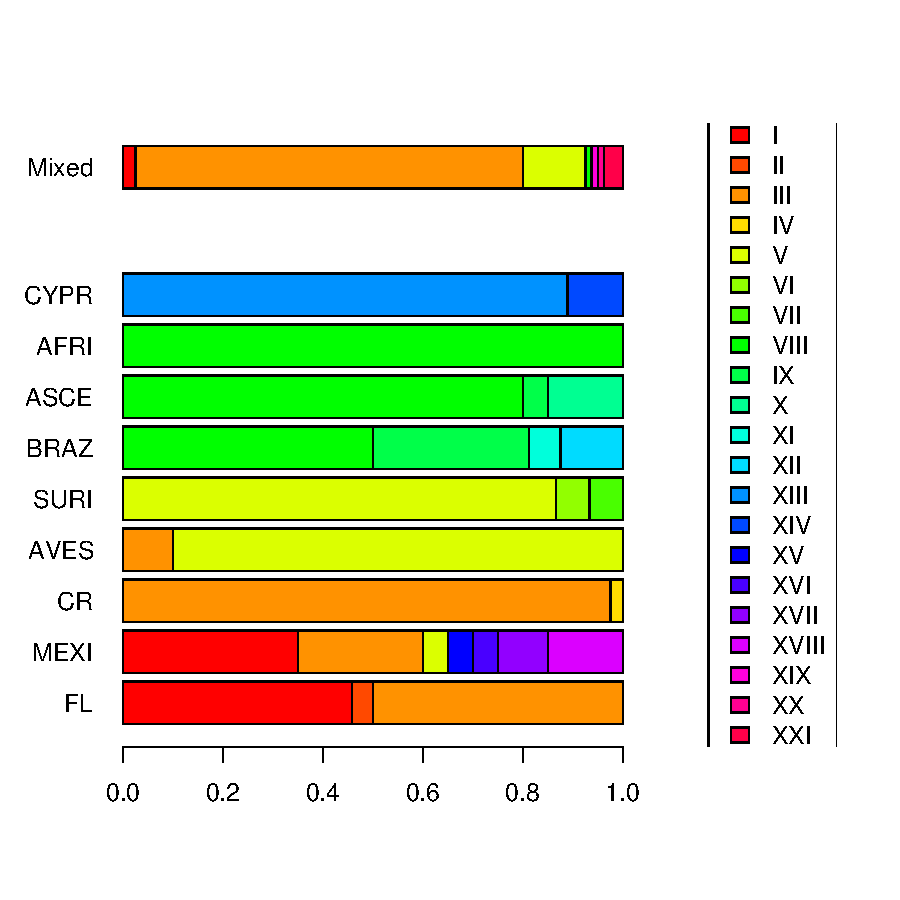
\includegraphics{mixstock-009}
\caption{Basic plot of turtle mtDNA haplotype data.}
\label{fig:data1}
\end{figure}

The default plot is a barplot, with the proportions of each haplotype
sampled in each rookery represented by a separate bar; the mixed
population data are shown as the rightmost bar.\footnote{you can
change from the default colors by specifying a {\tt colors=} argument:
e.g. if you have 10 haplotypes, {\tt colors=topo.colors(10)} or
{\tt colors=gray((0:9)/9)}. See {\tt ?gray} or {\tt ?rainbow} for
more information.}

Before proceeding, you will need to ``condense'' your data
set by (1) excluding any haplotype samples that are found only in the
mixed population (which will break some estimation methods, and
provide no useful information on turtle origins) and (2) lumping
together all haplotypes that are found only in a single rookery and
the mixed population (distinguishing among such haplotypes provides no
extra information in our analyses, and may slow down estimation).
You can do this by typing
\begin{Schunk}
\begin{Sinput}
> mydata <- markfreq.condense(mydata)
\end{Sinput}
\end{Schunk}
(To examine the condensed form of the data,
you can print them by typing \verb+mydata+ at
the command prompt, \verb+head(mydata)+ to see
just the first few lines, or \verb+plot(mydata)+ to see
the graphical summary [Figure~\ref{fig:condensed}].)

Some data are already entered in the package
in the condensed format; you can access them
using the {\tt data()} command.
\begin{Schunk}
\begin{Sinput}
> data(lahanas98)
\end{Sinput}
\end{Schunk}
makes the haplotype frequency data from Lahanas et al. 1998
\cite{Laha+98} available as variable {\tt lahanas98}.
\begin{Schunk}
\begin{Sinput}
> data(bolten98)
\end{Sinput}
\end{Schunk}
gives you the loggerhead data from Bolten et al. 1998
\cite{Bolt+98} available as {\tt bolten98},
already converted and condensed: {\tt bolten98raw}
gives you the raw table.

\begin{figure}
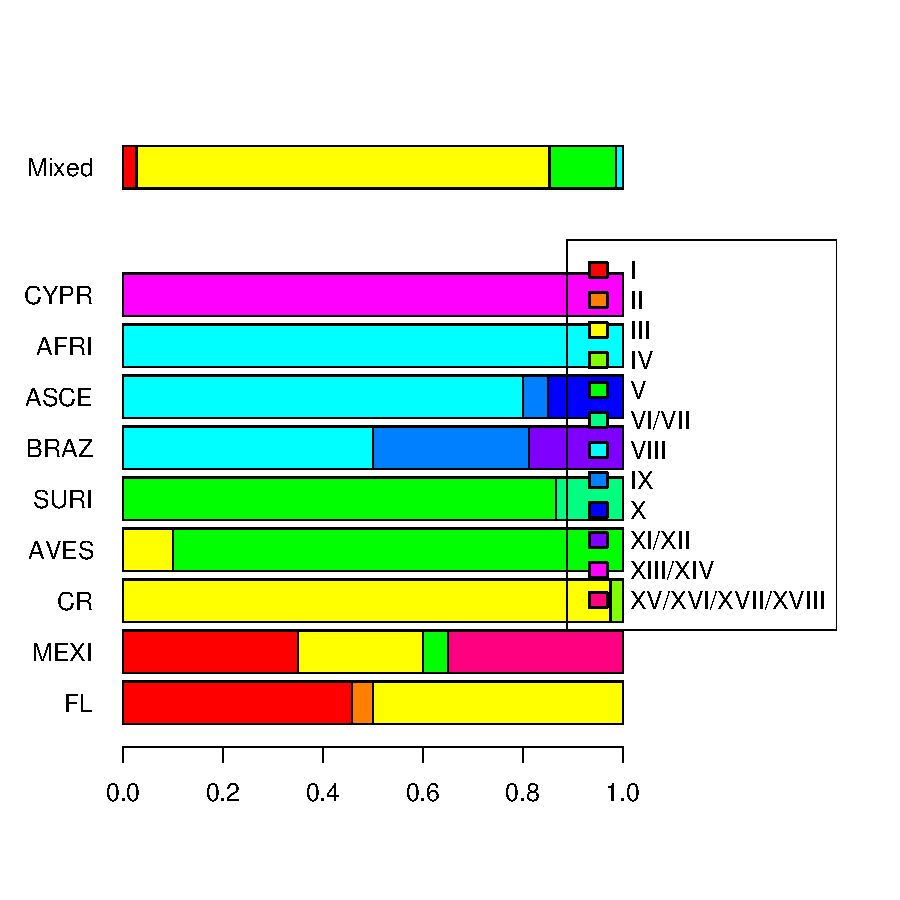
\includegraphics{mixstock-013}
\caption{Condensed haplotype data from Lahanas 1998}
\label{fig:condensed}
\end{figure}

\section{Stock analysis}
Various methods of stock analysis are available.

\subsection{Conditional and unconditional maximum likelihood}
You can do standard conditional maximum likelihood
(CML) analysis using \verb+cml(mydata)+.
If you want to save the results, you can save them
as a variable that you can then print, plot, etc.
(Figure~\ref{fig:cml1})
\begin{Schunk}
\begin{Sinput}
> mydata.cml <- cml(mydata)
> mydata.cml
\end{Sinput}
\begin{Soutput}
Estimated input contributions:
          FL         MEXI           CR         AVES         SURI         BRAZ 
5.463021e-02 9.453698e-05 7.833919e-01 1.485493e-01 1.333410e-06 1.333277e-06 
        ASCE         AFRI         CYPR 
1.333144e-06 1.332877e-02 1.333010e-06 

Estimated marker frequencies in sources:
(cml: no estimate)

method: cml 
\end{Soutput}
\end{Schunk}

\begin{Schunk}
\begin{Sinput}
> plot(mydata.cml)
\end{Sinput}
\end{Schunk}

\begin{figure}
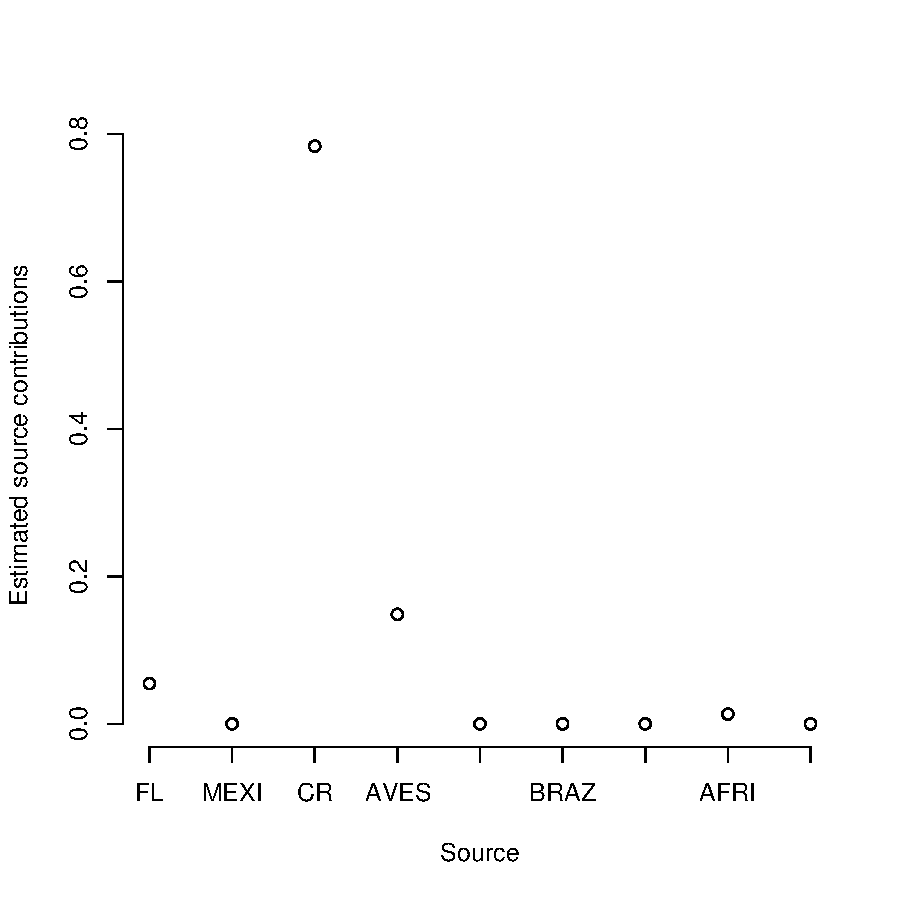
\includegraphics{mixstock-016}
\caption{CML estimates for Lahanas 1998 data}
\label{fig:cml1}
\end{figure}
When you print CML results, \R\ will tell you there is no estimate for
the rookery frequencies, because CML assumes that the true rookery
frequencies are equal to the sample rookery frequencies, rather than
estimating the rookery frequencies independently.

The default plot for estimation results plots
points specifying the estimated
proportions of the mixed population contributed by each
rookery (to plot this with a logarithmic scale
for the vertical axis, use
{\tt plot(mydata.cml,log="y")}).

Standard unconditional maximum likelihood analysis (UML)
takes a little longer, but is equally straightforward:
\begin{Schunk}
\begin{Sinput}
> mydata.uml <- uml(mydata)
\end{Sinput}
\end{Schunk}

UML estimates also include estimates of the true
haplotype frequencies in each rookery, which are
printed with the contribution estimates 
(print these results by typing {\tt mydata.uml} on a line by
itself).
As with CML, you can plot the results with
{\tt plot(mydata.uml)}; by default this plot
includes just the rookery contribution
information.
You can include the estimated haplotype
frequencies in the rookeries in the graphical summary as follows:
\begin{Schunk}
\begin{Sinput}
> par(ask = TRUE)
> plot(mydata.uml, plot.freqs = TRUE)
> par(ask = FALSE)
\end{Sinput}
\end{Schunk}
(The {\tt par} commands tell \R\ to wait
for user input, or not, between successive plots.)

\subsection{Confidence intervals:
CML and UML bootstrapping}
\begin{Schunk}
\begin{Sinput}
> mydata.umlboot <- genboot(mydata, "uml")
\end{Sinput}
\end{Schunk}
will generate standard (nonparametric)
bootstrap confidence intervals for
a UML fit to {\tt mydata}, by resampling
the data with replacement 1000 times (by default).
\emph{This is fairly slow with a realistic size
data set.}
(You can ignore warnings about {\tt singular matrix, returning
equal contribs}, {\tt Error in qr.solve}, etc..)
You can find out the results by typing
\begin{Schunk}
\begin{Sinput}
> confint(mydata.umlboot)
\end{Sinput}
\begin{Soutput}
                     2.5%        97.5%
contrib.FL   1.000000e-04 1.937642e-01
contrib.MEXI 8.172321e-05 9.999000e-05
contrib.CR   6.184032e-01 8.854842e-01
contrib.AVES 6.292138e-02 2.483440e-01
contrib.SURI 1.179836e-09 3.125456e-02
contrib.BRAZ 5.111485e-10 1.780757e-05
contrib.ASCE 1.598620e-13 2.008738e-05
contrib.AFRI 1.036273e-13 4.000358e-02
contrib.CYPR 1.779165e-13 2.142360e-05
\end{Soutput}
\end{Schunk}

\begin{figure}
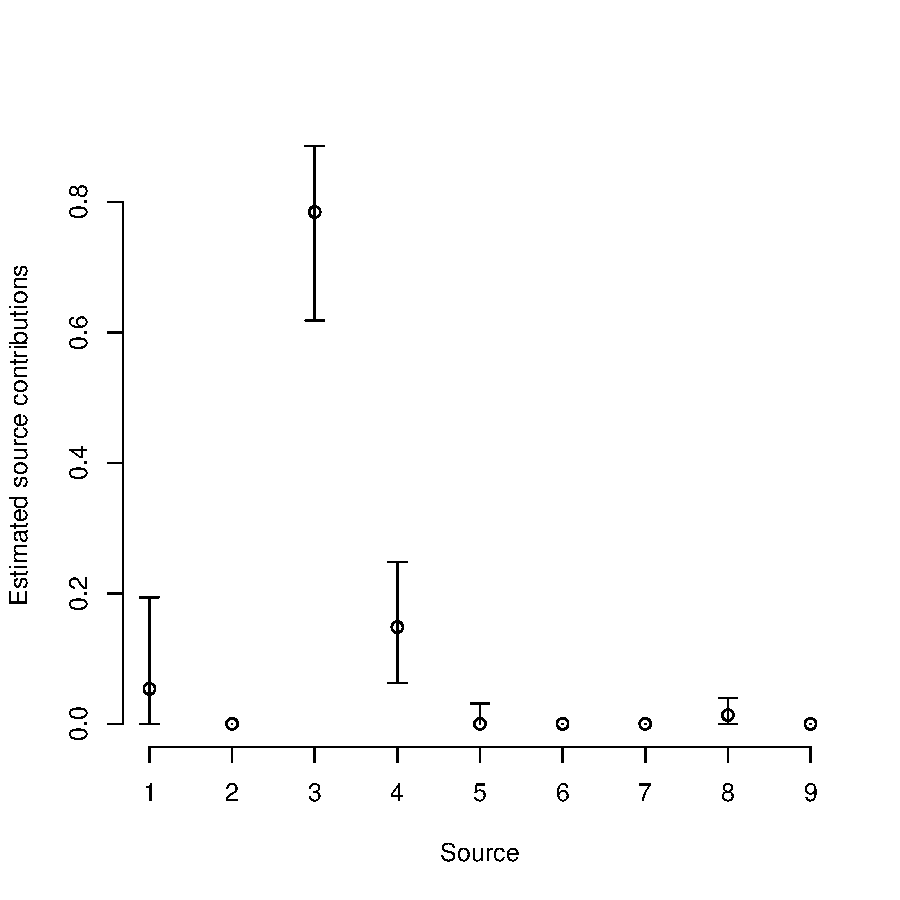
\includegraphics{mixstock-022}
\caption{UML estimates with bootstrap confidence limits for Lahanas 1998 data}
\label{fig:umlboot}
\end{figure}

\subsection{Markov Chain Monte Carlo estimation}
\begin{Schunk}
\begin{Sinput}
> mydata.mcmc <- tmcmc(mydata)
\end{Sinput}
\end{Schunk}

\begin{Schunk}
\begin{Sinput}
> mydata.mcmc
\end{Sinput}
\begin{Soutput}
Estimated input contributions:
  contrib.FL contrib.MEXI   contrib.CR contrib.AVES contrib.SURI contrib.BRAZ 
 0.055518267  0.009706668  0.777704826  0.105769897  0.036445990  0.003427765 
contrib.ASCE contrib.AFRI contrib.CYPR 
 0.004219192  0.005680010  0.001527386 

Estimated marker frequencies in sources:
NULL

method: mcmc 
prior strength: 0.1147742 
\end{Soutput}
\begin{Sinput}
> confint(mydata.mcmc)
\end{Sinput}
\begin{Soutput}
                     2.5%      97.5%
contrib.FL   2.009853e-11 0.23823757
contrib.MEXI 1.726347e-17 0.07512486
contrib.CR   5.956080e-01 0.89165907
contrib.AVES 3.616006e-10 0.22608667
contrib.SURI 7.363441e-16 0.17303709
contrib.BRAZ 1.664703e-16 0.02785796
contrib.ASCE 8.067783e-17 0.03001117
contrib.AFRI 3.820586e-15 0.03642586
contrib.CYPR 9.118769e-18 0.01506706
\end{Soutput}
\end{Schunk}
\begin{Schunk}
\begin{Sinput}
> plot(mydata.mcmc)
\end{Sinput}
\end{Schunk}

do the standard things: print the results, show confidence
intervals, plot the results.
(By default the information on haplotype frequencies
in rookeries is not saved --- it tends to be voluminous ---
and so this does not show up in the MCMC results.)

\begin{figure}
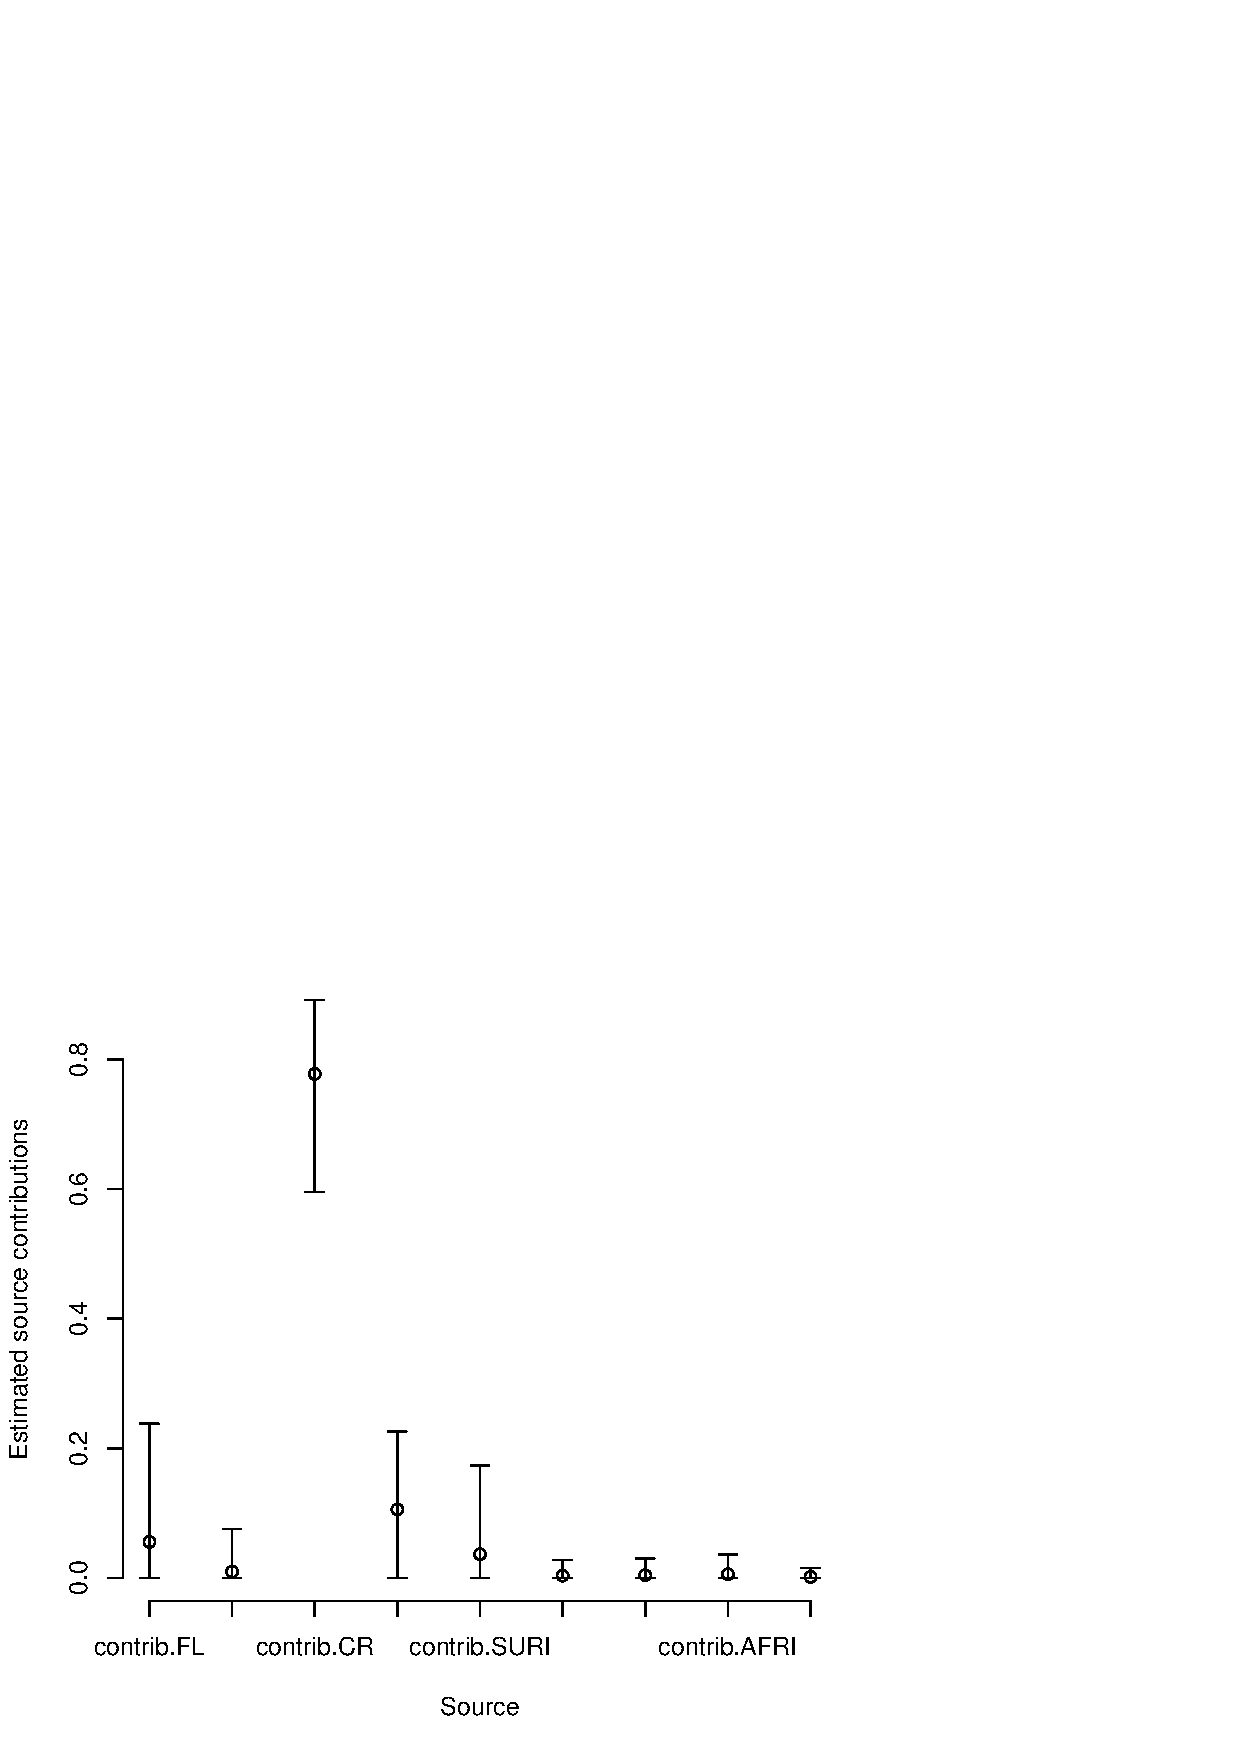
\includegraphics{mixstock-027}
\caption{MCMC estimates with confidence limits for Lahanas 1998 data}
\label{fig:mcmc1}
\end{figure}

\subsection{Convergence diagnostics for MCMC}

When you are running MCMC analyses, you have to check that
the Markov chains have \emph{converged} (i.e. that you've
run everything long enough for a reliable estimate).

\subsubsection{Raftery and Lewis}
The command
\begin{Schunk}
\begin{Sinput}
> diag1 = calc.RL.0(mydata)
\end{Sinput}
\end{Schunk}

runs \emph{Raftery and Lewis} diagnostics on your data
set: these criteria attempt to determine how long a single chain
has to be in order for it to give ``sufficiently good''
estimates.  This function actually runs an iterative
procedure, repeating the chain until the R\&L criterion
is satisfied.

The results consist of two parts:
\begin{itemize}
\item{\verb+diag1$current+ gives the 
diagnostics for the last chain evaluated.
These diagnostics consist of the
predicted required length of
the ``burn-in'' period (a transient that is discarded);
the total number of iterations required; a lower bound
on the total number required; and a ``dependence factor''
that tells how much correlation  there is between subsequent
values in the chain (see {\tt ?raftery.diag} for more
information).  Here are the first few lines
of \verb+diag1$current+:
\begin{Schunk}
\begin{Sinput}
> head(diag1$current)
\end{Sinput}
\begin{Soutput}
             Burn-in Total Lower bound Dependence factor
contrib.FL        18  1521         235              6.47
contrib.MEXI      14   926         235              3.94
contrib.CR        28  1804         235              7.68
contrib.AVES       4   312         235              1.33
contrib.SURI      15  1230         235              5.23
contrib.BRAZ       5   367         235              1.56
\end{Soutput}
\end{Schunk}
}
\item{
\verb+diag1$suggested+ gives the history of how
long each suggested chain was as we went along:
the iterations stop once suggested $>$current,
but note that there is a lot of variability in
the results.
\begin{Schunk}
\begin{Sinput}
> diag1$history
\end{Sinput}
\begin{Soutput}
iteration Current Suggested
        1     500       647
        2     647      3882
        3    3882      1804
\end{Soutput}
\end{Schunk}
}
\end{itemize}


\subsubsection{Gelman and Rubin}
The command
\begin{Schunk}
\begin{Sinput}
> diag2 = calc.GR(mydata)
\end{Sinput}
\end{Schunk}
tests the \emph{Gelman-Rubin} criterion, which starts multiple
chains from widely spaced starting points and tests to ensure
that the chains ``overlap'' --- i.e., that between-chain
variance is small relative to within-chain variance. 
The general rule of thumb is that the criterion should
be below 1.2 for all parameters in order for the chain
to be judged to have converged properly.
\cite{Gelm+96}.

\section{Hierarchical models}

To install {\tt WinBUGS}, go to
\url{http://www.mrc-bsu.cam.ac.uk/bugs/winbugs/contents.shtml}
and follow the instructions there to download and install {\tt WinBUGS} version 1.4
and get a license key.  Then make sure that you've installed
the {\tt R2WinBUGS} package.

You can use the {\tt pm.wbugs()} command (with the same syntax
as {\tt tmcmc} above) to run basic mixed stock analysis.
Use {\tt mm.wbugs()} to run many-to-many analyses.

\subsection{Many-to-many analysis}

The {\tt simmixstock2} command does basic simulation
of multiple-mixed-stock systems.  At its simplest,
it simply generates random uniform values for
the haplotype frequencies in each rookery
and the proportional contributions of each
rookery to each mixed stock:

\begin{Schunk}
\begin{Sinput}
> Z <- simmixstock2(nsource = 4, nmark = 5, nmix = 3, sourcesize = c(4, 
+     2, 1, 1), sourcesampsize = rep(25, 4), mixsampsize = rep(30, 
+     3), rseed = 1001)
> Z
\end{Sinput}
\begin{Soutput}
4 sources, 3 mixed stock(s), 5 distinct markers
Sample data:
   R1 R2 R3 R4 M1 M2 M3
H1 14  8  5 14 12  6  9
H2  2  0  0  0  3  4  1
H3  2  2 11  5  3  6  3
H4  2  2  7  0  4  6 10
H5  5 13  2  6  8  8  7
\end{Soutput}
\begin{Sinput}
> plot(Z)
\end{Sinput}
\end{Schunk}
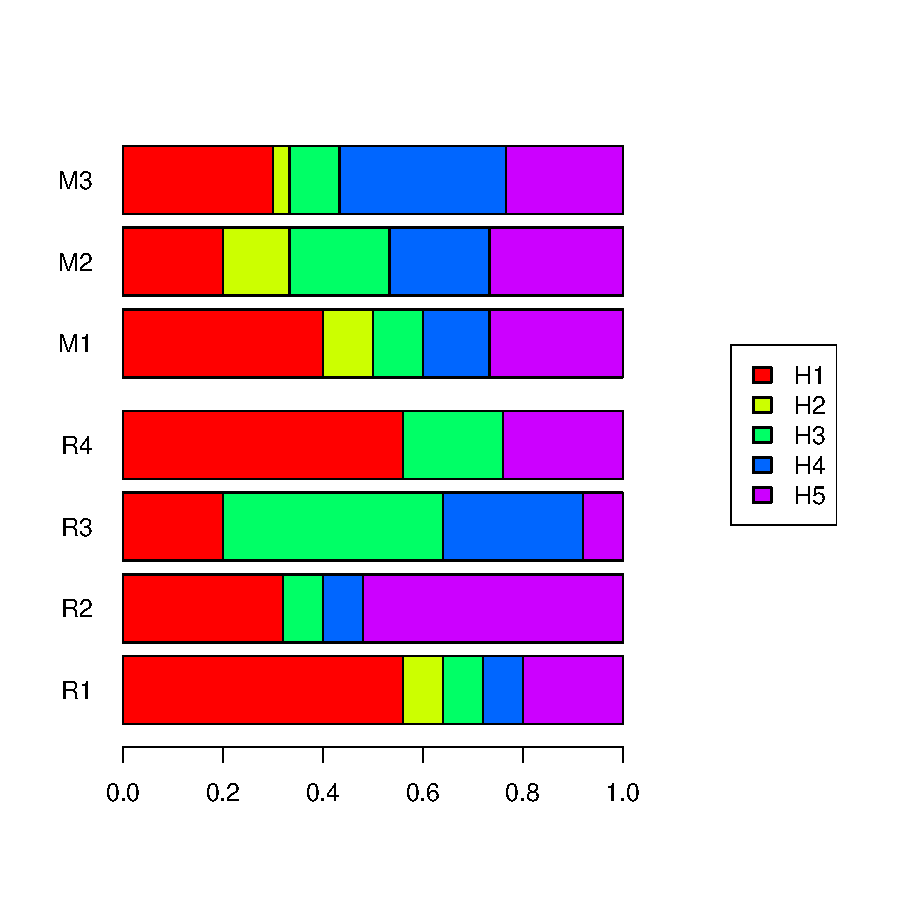
\includegraphics{mixstock-034}


Now try to fit this via {\tt mm.wbugs}:
\begin{Schunk}
\begin{Sinput}
> Zfit <- mm.wbugs(Z, sourcesize = c(4, 2, 1, 1))
\end{Sinput}
\end{Schunk}

Or, keeping the run in BUGS format for diagnostic purposes:
\begin{Schunk}
\begin{Sinput}
> Zfit0 <- mm.wbugs(Z, sourcesize = c(4, 2, 1, 1), returntype = "bugs")
\end{Sinput}
\end{Schunk}

This takes about 18.3 minutes to run with the
default settings, which run 4 chains (equal to the number of
sources) for 20,000 steps each.
(There are two different versions of the BUGS code that can
be used with {\tt mm.wbugs}; in this particular case they
give relatively similar answers and take about the same amount
of time ({\tt bugs.code="BB"} took 9.2 minutes), 
but if you're having trouble you might try switching
from the default {\tt bugs.code="TO"} to {\tt bugs.code="BB"}.

Other important options when running {\tt mm.wbugs} are:
\begin{itemize}
\item {\tt n.iter}: the default is 20,000 iterations per chain, with
  the first half used as burn-in ({\tt n.burnin=floor(n.iter/2)});
  this may be conservative, and could take a long time with
  realistically large data sets.  Use CODA's diagnostics as
  described above ({\tt raftery.diag}, {\tt gelman.diag}, etc.)
  to figure out an appropriate number of iterations.
\item {\tt n.chains}: equal to the number of sources by default,
  which may again be overkill.  (\cite{Bolker+07} used three chains
  for an 11-source problem.)
\item {\tt inittype}: {\tt "dispersed"} starts the chains from 
  a starting point where 95\% of the contributions are assumed to
  come from a single source; {\tt "random"} starts the chains from
  random starting points.  If {\tt which.init} is specified, these
  sources will be used as the dominant starting points: for example,
  {\tt mm.wbugs(...,n.chains=3,inittype="dispersed",which.init=c(1,5,7))} will 
  start 3~chains with dominant contributions from sources 1, 5, and 7.  If
  {\tt which.init} is unspecified and {\tt n.chains} is less than the
  number of sources, dominant sources will be picked at random.
\item {\tt returntype}: specifies what format to use for the answer.
  The default is a {\tt mixstock.est} object that can be plotted
  or summarized like the results from any other mixed-stock analysis.
  However, for diagnostic purposes, it may be worth running the
  code initially with {\tt returntype="bugs"}
  and using {\tt as.mcmc.bugs} and {\tt as.mixstock.est.bugs}
  to convert the result to either CODA format or mixstock
  format.  Plotting bugs format and CODA format gives different
  diagnostic plots; CODA format can also be used to run
  convergence diagnostics such as {\tt raftery.diag} or
  {\tt gelman.diag}.
\end{itemize}

Plots from many-to-many runs:

Plot BUGS format diagnostics (plot not shown):
\begin{Schunk}
\begin{Sinput}
> plot(Zfit0)
\end{Sinput}
\end{Schunk}

Plot CODA diagnostics (plot not shown):
\begin{Schunk}
\begin{Sinput}
> plot(as.mcmc.bugs(Zfit0))
\end{Sinput}
\end{Schunk}

Plot results:
\begin{Schunk}
\begin{Sinput}
> print(plot(Zfit))
\end{Sinput}
\end{Schunk}
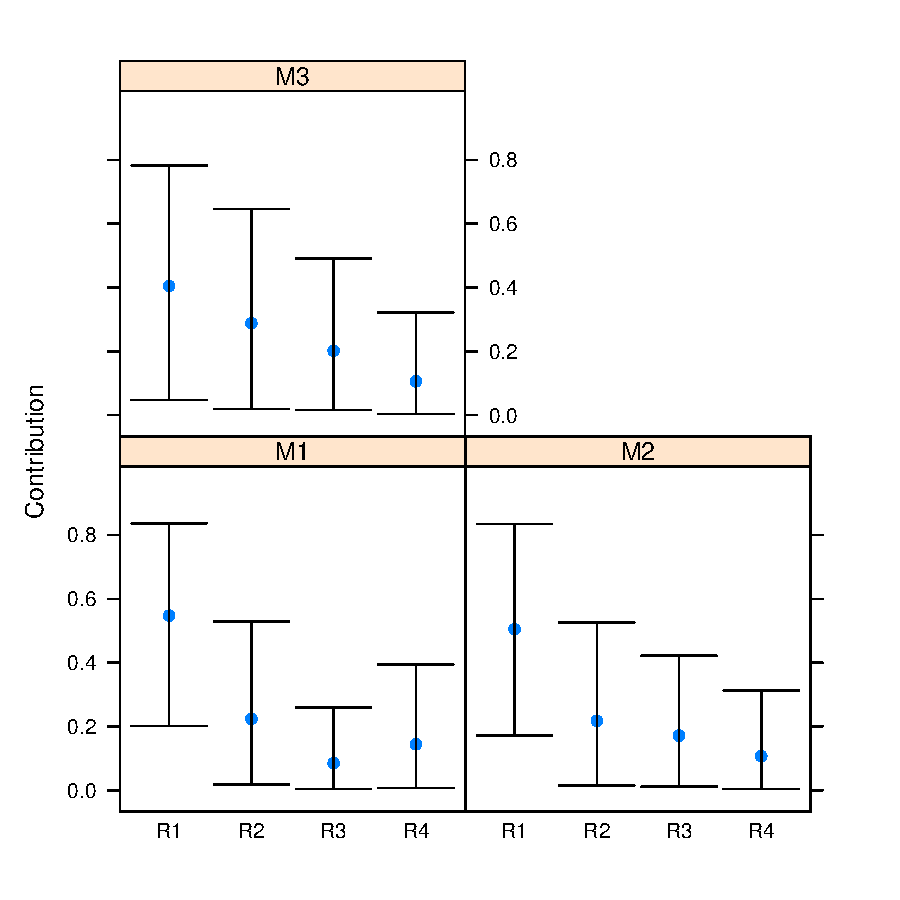
\includegraphics{mixstock-041}

Source-centric form:
\begin{Schunk}
\begin{Sinput}
> print(plot(Zfit, sourcectr = TRUE))
\end{Sinput}
\end{Schunk}
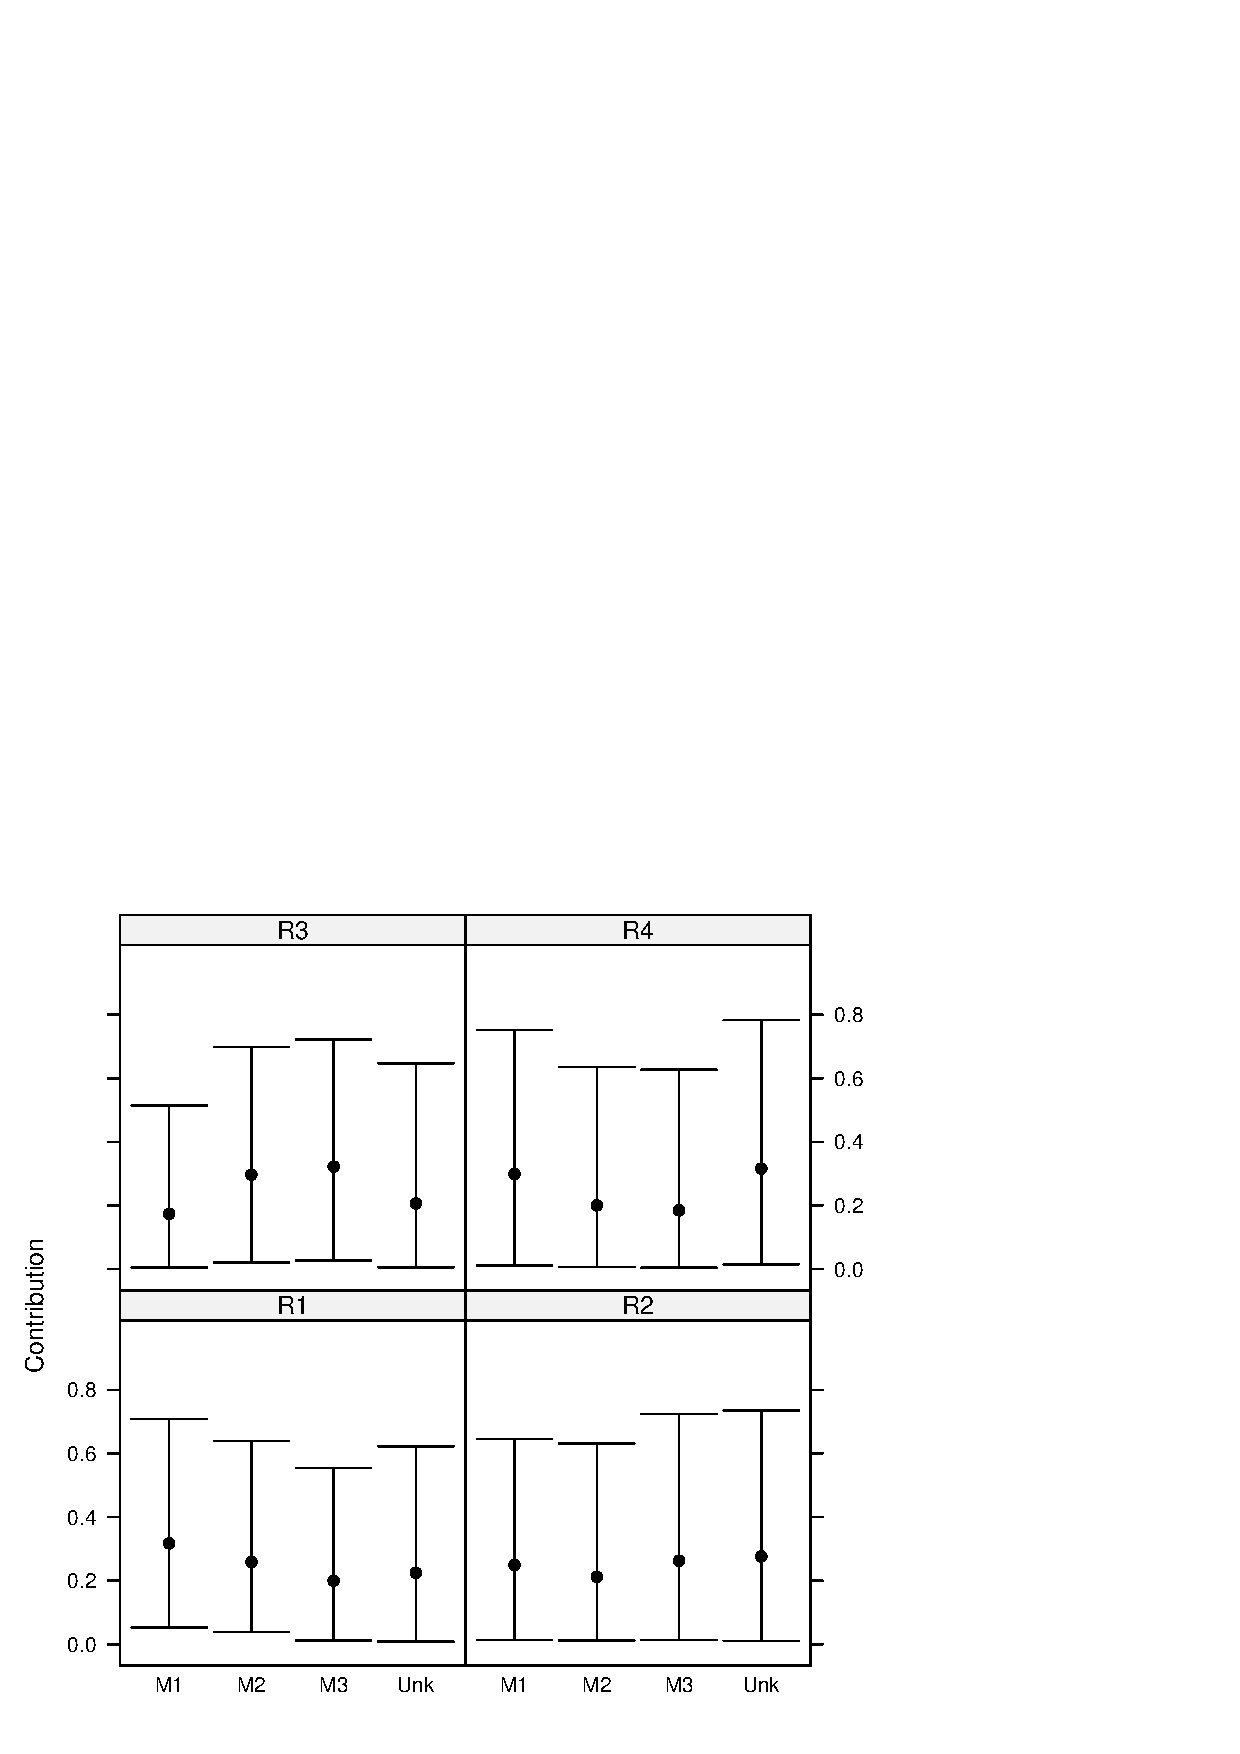
\includegraphics{mixstock-042}

Summary/confidence intervals:
\begin{Schunk}
\begin{Sinput}
> head(summary(Zfit))
\end{Sinput}
\begin{Soutput}
4 sources, 3 mixed stock(s), 5 distinct markers
Sample data:
   R1 R2 R3 R4 M1 M2 M3
H1 14  8  5 14 12  6  9
H2  2  0  0  0  3  4  1
H3  2  2 11  5  3  6  3
H4  2  2  7  0  4  6 10
H5  5 13  2  6  8  8  7

Estimates:

Mixed-stock-centric:
                       2.5%     97.5%
M1.R1 0.5473780 0.201795000 0.8366150
M1.R2 0.2235784 0.017553250 0.5286050
M1.R3 0.0850429 0.003377650 0.2590050
M1.R4 0.1440014 0.007369775 0.3941075
M2.R1 0.5043251 0.171260000 0.8346125
M2.R2 0.2178163 0.014860500 0.5255300
M2.R3 0.1712309 0.011442625 0.4215025
M2.R4 0.1066277 0.004133800 0.3124100
M3.R1 0.4046099 0.047320750 0.7818925
M3.R2 0.2877887 0.018549000 0.6452925
M3.R3 0.2017308 0.015441500 0.4913425
M3.R4 0.1058681 0.002893225 0.3213625

Source-centric:
                        2.5%     97.5%
R1.M1  0.3171615 0.052617250 0.7088300
R1.M2  0.2584727 0.038580500 0.6387150
R1.M3  0.1997042 0.012389250 0.5542900
R1.Unk 0.2246619 0.008175600 0.6225700
R2.M1  0.2492528 0.013269500 0.6460600
R2.M2  0.2118914 0.011240250 0.6314400
R2.M3  0.2626997 0.013295500 0.7239800
R2.Unk 0.2761556 0.010689750 0.7348300
R3.M1  0.1740109 0.005432050 0.5149200
R3.M2  0.2972163 0.020928500 0.6983675
R3.M3  0.3223322 0.026362250 0.7219875
R3.Unk 0.2064394 0.005509450 0.6473575
R4.M1  0.2988757 0.011309500 0.7524525
R4.M2  0.2004035 0.007036625 0.6351050
R4.M3  0.1847740 0.004338375 0.6272475
R4.Unk 0.3159484 0.015142750 0.7827350
$data
4 sources, 3 mixed stock(s), 5 distinct markers
Sample data:
   R1 R2 R3 R4 M1 M2 M3
H1 14  8  5 14 12  6  9
H2  2  0  0  0  3  4  1
H3  2  2 11  5  3  6  3
H4  2  2  7  0  4  6 10
H5  5 13  2  6  8  8  7

$fit
$fit$input.freq
          R1        R2        R3        R4
M1 0.5473780 0.2235784 0.0850429 0.1440014
M2 0.5043251 0.2178163 0.1712309 0.1066277
M3 0.4046099 0.2877887 0.2017308 0.1058681

$fit$source.freq
NULL

$fit$sourcectr.freq
          M1        M2        M3   Unknown
R1 0.3171615 0.2584727 0.1997042 0.2246619
R2 0.2492528 0.2118914 0.2626997 0.2761556
R3 0.1740109 0.2972163 0.3223322 0.2064394
R4 0.2988757 0.2004035 0.1847740 0.3159484


$resample.sum
            mean   median         sd       Q02.5       Q05      Q95     Q97.5
M1.R1  0.5473780 0.553600 0.16110594 0.201795000 0.2595000 0.799230 0.8366150
M1.R2  0.2235784 0.204450 0.13855505 0.017553250 0.0260570 0.474390 0.5286050
M1.R3  0.0850429 0.068225 0.06931447 0.003377650 0.0065684 0.233520 0.2590050
M1.R4  0.1440014 0.126050 0.10132943 0.007369775 0.0140235 0.334100 0.3941075
M2.R1  0.5043251 0.503550 0.16885282 0.171260000 0.2143150 0.782120 0.8346125
M2.R2  0.2178163 0.204700 0.13563086 0.014860500 0.0260610 0.468530 0.5255300
M2.R3  0.1712309 0.154500 0.10862593 0.011442625 0.0224255 0.379490 0.4215025
M2.R4  0.1066277 0.087870 0.08396023 0.004133800 0.0089415 0.272715 0.3124100
M3.R1  0.4046099 0.399100 0.20215962 0.047320750 0.0800140 0.738310 0.7818925
M3.R2  0.2877887 0.274750 0.17065027 0.018549000 0.0354680 0.596360 0.6452925
M3.R3  0.2017308 0.184400 0.12848814 0.015441500 0.0253800 0.435915 0.4913425
M3.R4  0.1058681 0.084805 0.08726567 0.002893225 0.0070214 0.287610 0.3213625
R1.M1  0.3171615 0.292000 0.17826667 0.052617250 0.0752155 0.651575 0.7088300
R1.M2  0.2584727 0.225500 0.16266044 0.038580500 0.0508010 0.574510 0.6387150
R1.M3  0.1997042 0.161000 0.15118056 0.012389250 0.0201575 0.504265 0.5542900
R1.Unk 0.2246619 0.185450 0.17268818 0.008175600 0.0161995 0.551420 0.6225700
R2.M1  0.2492528 0.221400 0.17715397 0.013269500 0.0206450 0.579150 0.6460600
R2.M2  0.2118914 0.175000 0.16305664 0.011240250 0.0201865 0.522395 0.6314400
R2.M3  0.2626997 0.223000 0.19132121 0.013295500 0.0223965 0.634180 0.7239800
R2.Unk 0.2761556 0.241950 0.19892308 0.010689750 0.0219895 0.644830 0.7348300
R3.M1  0.1740109 0.135750 0.14152211 0.005432050 0.0128130 0.451170 0.5149200
R3.M2  0.2972163 0.272700 0.18146115 0.020928500 0.0434125 0.629540 0.6983675
R3.M3  0.3223322 0.298150 0.19033388 0.026362250 0.0460470 0.656430 0.7219875
R3.Unk 0.2064394 0.158350 0.17602759 0.005509450 0.0108000 0.571265 0.6473575
R4.M1  0.2988757 0.256650 0.20717218 0.011309500 0.0235090 0.687640 0.7524525
R4.M2  0.2004035 0.150150 0.16932025 0.007036625 0.0121855 0.531450 0.6351050
R4.M3  0.1847740 0.134400 0.16408396 0.004338375 0.0093100 0.520820 0.6272475
R4.Unk 0.3159484 0.269400 0.21798576 0.015142750 0.0292240 0.729235 0.7827350
\end{Soutput}
\end{Schunk}
(check this!)

\section{Quick start}
\label{sec:quickstart}
\begin{itemize}
\item{Download and install \R\ from
CRAN (find the site closest to you
at \url{http://cran.r-project.org/mirrors.html};
go to ``Precompiled binary distributions'' and
from there to the base package; pick
your operating system; download the setup 
program; and run the setup program).
}
\item{Start \R.}
\item{From within \R,
download and install the {\tt mixstock}
package and auxiliary packages:
\begin{Schunk}
\begin{Sinput}
> bbcontrib <- "http://www.zoo.ufl.edu/bolker/R/windows"
> install.packages("mixstock", contriburl = bbcontrib)
> install.packages("plotrix")
> install.packages("coda")
> install.packages("abind")
> install.packages("R2WinBUGS")
\end{Sinput}
\end{Schunk}
(This installation procedure needs to be done
only once, although the {\tt library} command
below, loading the package, needs to be done for every new R session.)
}
\item{Load the package: {\tt library(mixstock)}}
\item{Load data from a comma-separated value (CSV) file,
convert to proper format, and condense haplotypes:
\begin{Schunk}
\begin{Sinput}
> mydata <- hapfreq.condense(as.mixstock.data(read.csv("myfile.dat")))
\end{Sinput}
\end{Schunk}
} 
\item{analyze, e.g:
\begin{Schunk}
\begin{Sinput}
> mydata.mcmc <- tmcmc(mydata)
> mydata.mcmc
> intervals(mydata.mcmc)
> plot(mydata.mcmc)
\end{Sinput}
\end{Schunk}
}
\end{itemize}

\section{To do}
\begin{itemize}
\item{read.csv/read.table + as.mixstock.data combined
into a single read.mixstock.data command? (also incorporate
hapfreq.condense as a default option)}
\item{{\tt print.mixstock.est} could print sample frequencies instead of
saying ``no estimate'' for CML}
\item{MCMC section could be cleaned up considerably, explained better,
R\&L parameters not hard-coded, more efficient --- don't
re-run chains every time}
\item{incorporate rookery sizes in data}
\item{keep CODA objects or potential for CODA plots in MCMC results}
\item{make MCMC convergence process more efficient: more explanation}
\item{add hierarchical models????}
\item{describe fuzz and bounds parameters on CML/UML,
E-M algorithm}
\item{plot(...,legend=TRUE) doesn't work for CML.
add unstacked/beside=TRUE option to plot.mixstock.est}
\item incorporate source size data as part of data object
\item some functions don't work with uncondensed data: fix or issue warning
\item use {\tt HPDinterval} from CODA for confidence intervals,
  rather than quantiles?
\end{itemize}

\bibliography{mixstock}
\end{document}

